\frametitle{Receptor}
The B-DNA dodecamer d(CGCGAATTCGCG) described by James Watson and Francis Crick The double helix makes one complete turn about its axis every 10.4–10.5 base pairs in solution. This frequency of twist (termed the helical pitch) depends largely on stacking forces that each base exerts on its neighbours in the chain. \begin{wrapfigure}{r}{0.5\textwidth}
	\vspace{-2em}
	\begin{center}
		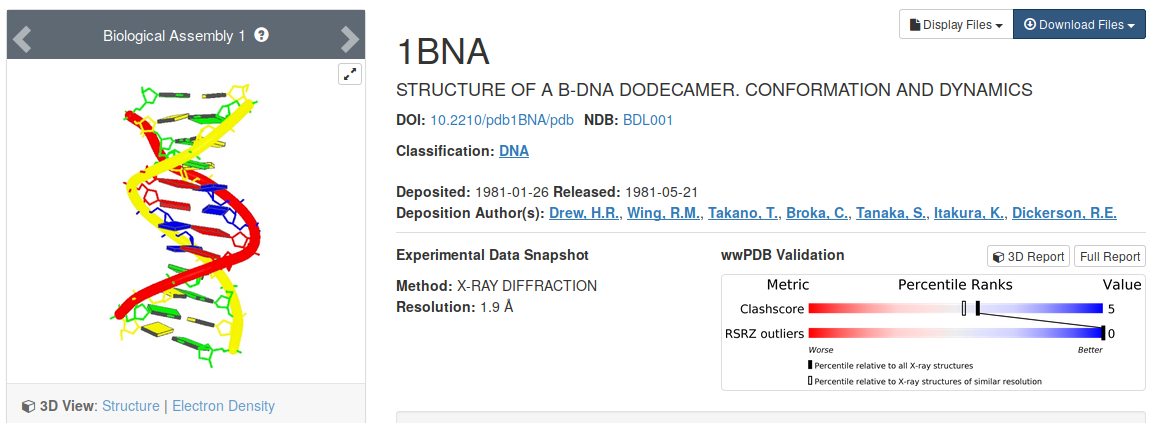
\includegraphics[width=0.5\textwidth]{receptor.png}
	\end{center}
\end{wrapfigure}The absolute configuration of the bases determines the direction of the helical curve for a given conformation. The 3D structure of a B-DNA dodecamer containing the atom count of 486 with the 1.9Å was obtained from the PDB (PDB: 1BNA) \cite{drew1981structure}.
